\section{Channel models}

The \acrfull{nlse} and the \acrfull{me} are two commonly used mathematical models for describing the behavior of light propagation in a single-mode optical fiber, including the effects of dispersion and nonlinearity~\cite{Agrawal2010}.
The \acrshort{nlse}, being a generic model describing the interplay between the dispersive and nonlinear effects, is applicable to the description of a vast number of physical phenomena, ranging from the dynamics of magneto-ordered systems \cite{kik90} to hydrodynamics \cite{o10}. It also serves, under certain assumptions, as a principal master model governing the evolution of a single-polarisation slow-varying light envelope propagating along the single-mode fibre \cite{a12,mg06}. In the context of optical fiber transmission, the Schr\"odinger equation is used to describe the evolution of the slowly varying optical field envelope, $A(z,t)$, in the presence of dispersion and nonlinearity. The general form of the Schr\"odinger equation for a single-polarization signal is as follow:

\begin{equation}
	\frac{\partial A }{\partial z} = - \frac{\alpha}{2} A - i \frac{\beta_2}{2} \frac{\partial^2 A}{\partial t^2} + i \gamma |A|^2 A {,}
\label{eq:nlse_att}
\end{equation}
where $z$ represents the distance along the fiber, $t$ is time, $\beta_2$ is the group velocity dispersion (GVD) parameter, $\gamma$ is the nonlinear coefficient, and $A$ is the complex envelope of the optical field.

The Manakov equation is a more complex model that is used to describe the behaviour of light propagation in a two-polarisation optical fiber. It considers the effects of polarization-mode dispersion and nonlinear interactions between the two polarizations. The Manakov equation for a two-polarization signal is as follows:
\begin{gather} 
\frac{\partial A_x}{\partial z} = -\frac{\alpha}{2} A_x - i\frac{\beta_2}{2}\frac{\partial^2 A_x}{\partial t^2} + i\gamma\frac{8}{9}\left(|A_x|^2 + |A_y|^2\right) A_x {,} \nonumber \\
\frac{\partial A_y}{\partial z} = -\frac{\alpha}{2} A_y - i\frac{\beta_2}{2}\frac{\partial^2 A_y}{\partial t^2} + i\gamma\frac{8}{9}\left(|A_x|^2 + |A_y|^2\right) A_y {,}
\label{eq:manakov_att}
\end{gather}
where $A_x$ and $A_y$ are the complex envelopes of the two polarizations. 
This model includes attenuation and is applied in simulations of \Gls{edfa}. 

It is important to specifically address the scenario where \(\alpha = 0\), which is relevant for \Gls{nft} systems and their analysis. The use of \gls{nft} in the presence of attenuation necessitates extra steps, including the estimation of an effective nonlinear coefficient \(\gamma_{\text{eff}}\). While this discussion is outside the current document's focus, it certainly represents a promising area for future research that could build upon the findings presented here.


In this study, we have simplified the channel model to exclude attenuation, a necessary simplification for applying \Gls{nft} to optical communications signals. The \Gls{nlse} for a channel model without attenuation is presented in dimensioned units as:
\begin{equation}
    i\frac{\partial A }{\partial z} - \frac{\beta_2}{2} \frac{\partial^2 A}{\partial t^2} + \gamma |A|^2 A = 0,
\label{eq:nlse}
\end{equation}
To effectively utilize \Gls{nft}, we introduce non-dimensional variables using characteristic scales like the pulse width or symbol interval \( T_0 \), dispersion length \( L_D = T_0^2/|\beta_2| \), and characteristic power \( P_0=1/(\gamma L_D) \). These lead to the following dimensionless equation, where \( \sigma \) represents either focusing (\( \sigma = 1 \)) or defocusing (\( \sigma = -1 \)) dispersion:
\begin{equation}
    i \frac{\partial q }{\partial \zeta} + \frac{\sigma}{2} \frac{\partial^2 q}{\partial \tau^2} +  |q|^2 q = 0,
\label{eq:nlse_norm}
\end{equation}



% %TODO: add normalisation and say that there are two ways to normilise
% For channel model without attenuation \Gls{nlse} in dimension units have the following form:
% \begin{equation}
% 	i\frac{\partial A }{\partial z} - \frac{\beta_2}{2} \frac{\partial^2 A}{\partial t^2} + \gamma |A|^2 A = 0 {,}
% \label{eq:nlse}
% \end{equation}

% It is convenient to introduce the characteristic time scale, e.g. carrier pulse width or symbol interval $T_0$, dispersion length $L_D = T_0^2/|\beta_2|$ and characteristic power $P_0=1/(\gamma L_D)$ to define corresponding non-dimensional variables $\tau=t/T_0$, $\zeta=z/L_D$ and $q=A/\sqrt{P_0}$. In dimensionless form the coefficient $\sigma$ defines focusing (anomalous dispersion, $\sigma = 1$) and defocusing (normal dispersion, $\sigma = -1$) cases.
% \begin{equation}
% 	i \frac{\partial q }{\partial \zeta} + \frac{1}{2} \frac{\partial^2 q}{\partial \tau^2} + \sigma |q|^2 q = 0 {,}
% \label{eq:nlse_norm}
% \end{equation}


In the situation where there is no signal loss ($\alpha = 0$), the \Gls{me} equations are:
\begin{gather} 
i \frac{\partial A_x}{\partial z} - \frac{\beta_2}{2}\frac{\partial^2 A_x}{\partial t^2} + \gamma\frac{8}{9}\left(|A_x|^2 + |A_y|^2\right) A_x = 0, \nonumber \\
i \frac{\partial A_y}{\partial z} - \frac{\beta_2}{2}\frac{\partial^2 A_y}{\partial t^2} + \gamma\frac{8}{9}\left(|A_x|^2 + |A_y|^2\right) A_y = 0,
\label{eq:manakov}
\end{gather}
with the same symbol interval \( T_0 \), the dispersion length \( L_D = T_0^2/|\beta_2| \) reference power level now scaled with \( P_0=1/(\frac{8}{9} \gamma L_D) \). These choices allow us to define scaled variables \( \tau=t/T_0 \), \( \zeta=z/L_D \), and \( q_{x,y}=A_{x,y}/\sqrt{P_0} \):
\begin{gather} 
i \frac{\partial q_x}{\partial \zeta} + \frac{\sigma}{2}\frac{\partial^2 q_x}{\partial \tau^2} +  \left(|q_x|^2 + |q_y|^2\right) q_x = 0, \nonumber \\
i \frac{\partial q_y}{\partial \zeta} + \frac{\sigma}{2}\frac{\partial^2 q_y}{\partial \tau^2} + \left(|q_x|^2 + |q_y|^2\right) q_y = 0.
\label{eq:manakov_norm}
\end{gather}
For clarity, throughout this paper, we will refer to the scaled fields \( q \) (from \( A \)) or \( q_{x,y} \) (from \( A_{x,y} \)) simply as 'the signal'.



% For \Gls{me} in case without attenuation $\alpha = 0$:
% \begin{gather} 
% i \frac{\partial A_x}{\partial z} - \frac{\beta_2}{2}\frac{\partial^2 A_x}{\partial t^2} + \gamma\frac{8}{9}\left(|A_x|^2 + |A_y|^2\right) A_x = 0 {,} \nonumber \\
% i \frac{\partial A_y}{\partial z} - \frac{\beta_2}{2}\frac{\partial^2 A_y}{\partial t^2} + \gamma\frac{8}{9}\left(|A_x|^2 + |A_y|^2\right) A_y = 0 {,}
% \label{eq:manakov}
% \end{gather}
% we can make almost same change of variables symbol interval $T_0$, dispersion length $L_D = T_0^2/|\beta_2|$ and characteristic power $P_0=1/(\frac{8}{9} \gamma L_D)$ to define corresponding non-dimensional variables $\tau=t/T_0$, $\zeta=z/L_D$ and $q_{x,y}=A_{x,y}/\sqrt{P_0}$:
% \begin{gather} 
% i \frac{\partial q_x}{\partial \zeta} + \frac{1}{2}\frac{\partial^2 q_x}{\partial \tau^2} + \sigma \left(|q_x|^2 + |q_y|^2\right) q_x {,} \nonumber \\
% i \frac{\partial q_y}{\partial \zeta} + \frac{1}{2}\frac{\partial^2 q_y}{\partial \tau^2} + \sigma \left(|q_x|^2 + |q_y|^2\right) q_y {.}
% \label{eq:manakov_norm}
% \end{gather}
% Without loss of generality, we will refer in the paper to the field $q$ ($A$) or $q_{x,y}$ ($A_{x,y}$) as to ``a signal''.


For the \gls{nft}, we work with the \gls{nlse} and the \gls{me} as set out in Eqs.~(\ref{eq:nlse_norm}) and~(\ref{eq:manakov_norm}). It's important to note that we can adjust the equations using a normalization factor of 2. This means setting the dispersion length \( L_D \) and the characteristic power \( P_0 \) as \( L_D = 2 T_0^2/|\beta_2| \) and \( P_0=2/(\frac{8}{9} \gamma L_D) \), respectively. After normalization, the fields \( q_{x,y}=A_{x,y}/\sqrt{P_0} \) for dual-polarization or simply \( q=A/\sqrt{P_0} \) for a single polarization remain the same. The normalized \acrlong{nlse} and \acrlong{me} equations are then written as:
\begin{equation}
	\frac{\partial q }{\partial \zeta} + \sigma \frac{\partial^2 q}{\partial \tau^2} + 2 |q|^2 q = 0,
\label{eq:nlse_norm2}
\end{equation}
for a single polarisation, and for dual polarisation:
\begin{gather} 
i \frac{\partial q_x}{\partial \zeta} + \sigma\frac{\partial^2 q_x}{\partial \tau^2} + 2 \left(|q_x|^2 + |q_y|^2\right) q_x = 0, \nonumber \\
i \frac{\partial q_y}{\partial \zeta} + \sigma\frac{\partial^2 q_y}{\partial \tau^2} + 2 \left(|q_x|^2 + |q_y|^2\right) q_y = 0,
\label{eq:manakov_norm2}
\end{gather}
respectively.


% -----------------------------------------------------------------------
% -----------------------------------------------------------------------
% -----------------------------------------------------------------------
% Nonlinear Fourier Transform
% -----------------------------------------------------------------------
% -----------------------------------------------------------------------
% -----------------------------------------------------------------------

\section{Nonlinear Fourier Transform}

\subsection{Introduction}

Quite often, the evolution of nonlinear systems is well approximated by the nonlinear partial differential equations (PDE). Evidently, there is no universal theory for the solution of nonlinear PDEs, but there exists a distinguished class of nonlinear equations that can be solved with a mathematical rigour: the so-called integrable systems. The history of integrable PDEs started in the 1960s when Gardner et al. \cite{ggk67} discovered a method for finding the infinite families of exact solutions for the  Korteweg-de Vries equation. Their method termed the inverse scattering transform, can be deemed as the generalisation of the conventional Fourier transform (FT) to the nonlinear systems. Thus, the name nonlinear Fourier transform (NFT) for it is often used nowadays, especially in the signal processing literature \cite{yk14-1,tplwfkd17}. Shortly after the integration of the Korteweg-de Vries equation, Zakharov and Shabat developed the inverse scattering machinery (i.e. the NFT method) for yet another celebrated PDE: the nonlinear Schr\"odinger equation (NLSE) \cite{zs72}, which will be the focus of our current study.  

In a nutshell, for an integrable PDE there exists the canonical transform of dependent variables, converting the original nonlinear system into the so-called action-angle variables; the evolution of the latter is governed by a set of uncoupled trivial (linear) differential equations. Mathematically, this can be treated as the effective linearisation of a nonlinear integrable PDE \cite{akn74,nmp84}. For our work, it is important that we know the explicit form of the NFT operations attributed to the NLSE.

Withing modern optical communications, the NFT is used not as a tool for the NLSE solution, but as a signal processing method \cite{tplwfkd17,yk14-1}. This concept originated from the work of Hasegawa and Nyu \cite{hn93}, who proposed to depart from considering the time domain solitonic shapes \cite{mg06}, but rather use the nonlinear spectrum (the so-called eigenvalues) for the data modulation and transmission. Over the last decade, the NFT-based optical transmission techniques have been resurrected and greatly extended~\cite{tplwfkd17,yal19}. The most efficient NFT-based optical transmission method is the so-called nonlinear frequency division multiplexing (NFDM) \cite{yk14-1}, within which we directly modulate the parameters of the nonlinear modes that emerge from the nonlinear Fourier (NF) signal decomposition. When the optical field propagates down the fibre link, the evolution of the nonlinear modes inside the NF domain stays almost linear, in contrast to the truly nonlinear evolution of signal in the space-time domain. Due to this property, we can theoretically get rid of the infamous nonlinear cross-talk degrading the transmission performance at high signal powers\cite{ekw10}. 

Generally, when considering the NF decomposition of an arbitrary rapidly decaying wave-form, we can have two distinct coexisting parts of the NF spectrum: the continuous part, describing quasi-linear dispersive waves, and the discrete part, corresponding to solitonic modes \cite{nmp84,akn74,tplwfkd17,yk14-1}. The continuous part of NF spectrum is represented by the complex-valued function $r(\xi) \in \mathbb{C}$ of a real argument $\xi \in \mathbb{R}$, where $\xi$ is called the spectral parameter; $r(\xi)$ is called the reflection coefficient, and $\xi$ emerges as the nonlinear analogue of a conventional Fourier frequency. This NF spectrum part converges to the conventional FT of our signal in the low-power limit \cite{pdt13}. The discrete part consists of the complex eigenvalues $\xi_n \in \mathbb{C}^{+}$, located in the upper complex half-plane, and the associated norming constants $r_n$ (spectral amplitudes) \cite{a16}. The graphical summary of the general NF spectrum structure is given in Fig.~\ref{fig:spectrum_representation}. However, we point out that it is exactly the utilisation of the continuous NF spectrum part \cite{pdbgt14,lpt14,lpt15,lpr15,lpphet16,lab17,kplt17_2,yy19} that resulted in the breakthrough in the NFDM technology: this idea, mentioned already in early NFT transmission-related works \cite{yk14-1,pdt13}, is in stark contrast with the progenitor soliton-based transmission methods~\cite{mg06}. We mention that the continuous NF spectrum modulation using the special technique coined b-modulation \cite{w17,gzl18,svp20,cw20} has provided the highest NFDM data rates so far \cite{yal19,yla19}.  Finally, we note that for the NFDM based on the discrete NF spectrum \cite{hyk16,bai16,wxz20}, the achieved data rates have been noticeably lower than those for the modulation of continuous NF spectrum, see the comparison in \cite[Fig. 1]{yal19}.
\begin{figure}[tbh]
    \centering
    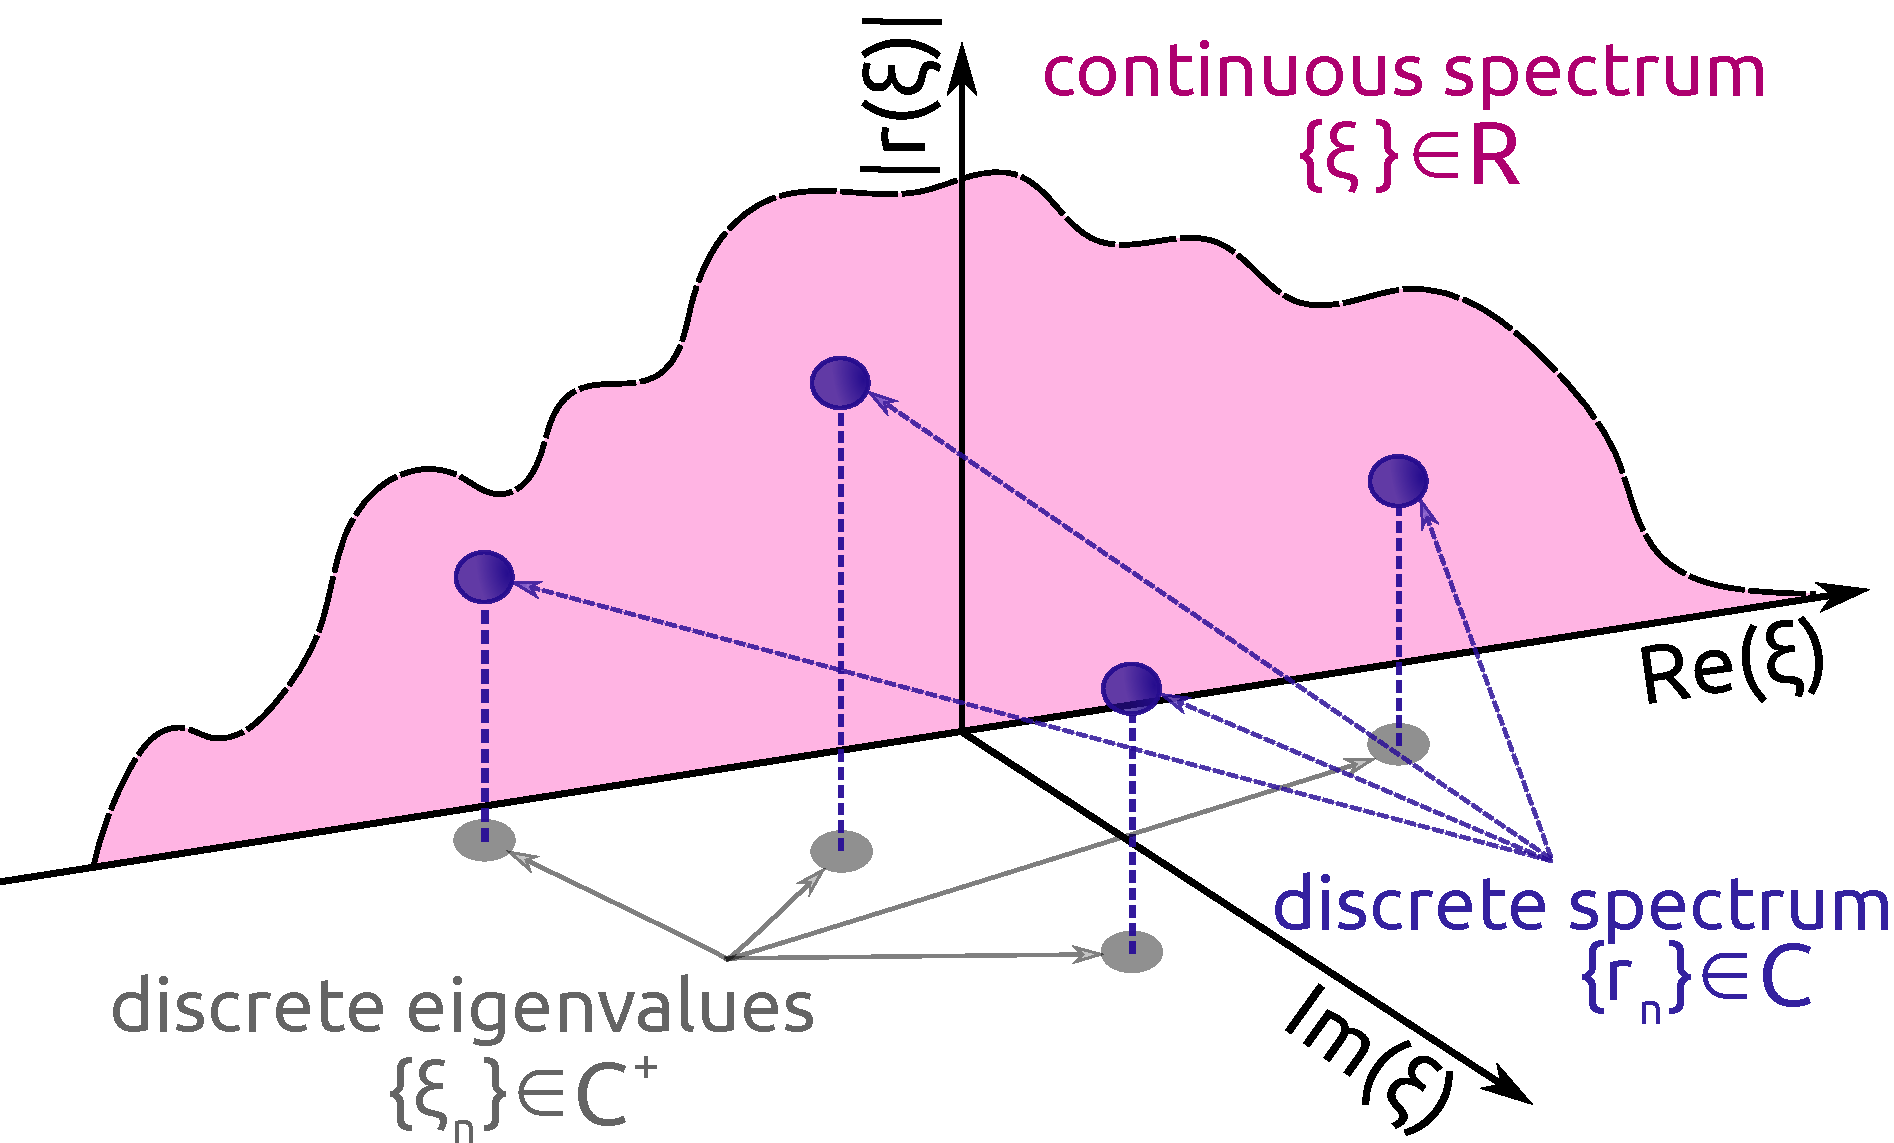
\includegraphics[width=0.55\linewidth]{images/nn_nft/nft_spectrum_representation_6.pdf}
    \caption{The schematic showing the different coexisting parts of a general NF spectrum: the discrete part, represented by the eigenvalues $\xi_n$ and respective norming constants $r_n$, and the continuous part, shown as the function $|r(\xi)|$ on the real $\xi$-axis. }
    \label{fig:spectrum_representation}
\end{figure}

The NFDM transmission method relies on the (approximate) integrability of our transmission channel, i.e. we inherently assume that Eq.~(\ref{eq:nlse_norm}) is a very accurate model describing the signal evolution down the fibre. However, aside from second-order dispersion and Kerr nonlinearity present in (\ref{eq:nlse_norm}), in realistic fibre-optic systems, there are numerous other effects affecting signal's propagation. Optical noise inevitably arising during the amplification process \cite{a12} is one of the key challenges in optical communications. The noise results in random NF spectrum disturbances \cite{dpt16,pvd20}, imposing limits on the NFDM transmission quality.  Another widespread deviation from idealised model (\ref{eq:nlse_norm}) is the non-zero nonuniform gain-loss profile occurring in realistic systems for both lumped \cite{lpt15,kplt17_2} and distributed \cite{lpr15} amplification schemes. We also mention the effects of polarisation mode dispersion \cite{ylb17,ts19}, higher-order chromatic dispersion \cite{ylb17}, and component-induced impairments, to itemise just several important sources. All these effects bring about the deviations of the true optical channel from integrable NLSE (\ref{eq:nlse_norm}) such that the NF spectrum of the signal at the end of our transmission system can be significantly distorted, which results in the appearance of errors in the transmitted data \cite{lpphet16,lab17,ylb17}.  Given that,  the machine learning and artificial neural networks (NN) based signal processing methods have recently attracted much attention, as they can effectively render adaptive distortions-resilient signal processing tools, and, thus, using the NNs we can mitigate the impact of detrimental factors mentioned above \cite{mrn18,kfl19}.  


Finally, we note that, recently, the interest in using the NFT as a signal-processing tool has risen in fields that are not directly relevant to optical transmission. In particular, the NFT was applied in the so-called integrable turbulence to monitor the appearance of coherent structures, such as breathers, solitons, and rogue waves \cite{rsc18,sda16}, to the optical microresonators regime analysis \cite{tcf20}, to the optical frequency combs characterisation \cite{wsh20}, and to the analysis of laser regimes and the emergence of dissipative coherent nonlinear structures \cite{rnb18,skp19,csf19}. The analysis of NFT modes' evolution for such systems often appears to be more informative and convenient than dealing with the conventional Fourier modes. The NFT is also an important tool for the design of fibre Bragg gratings \cite{FBG01,FBG02}. Thus, we believe that the technique presented in this work can have a much wider range of applications than simply being a processing tool in optical communications. To end up, solving nonlinear differential equations itself by using NNs is a fast-growing area with a range of applications in science and engineering \cite{rbp17,lkb18,lka20}. We hope that our work will also advance knowledge in this emerging field.

\subsection{Theory}

\subsubsection{\acrshort{nft} for \acrlong{nlse}}

\begin{figure}[tbp]
	\centering
	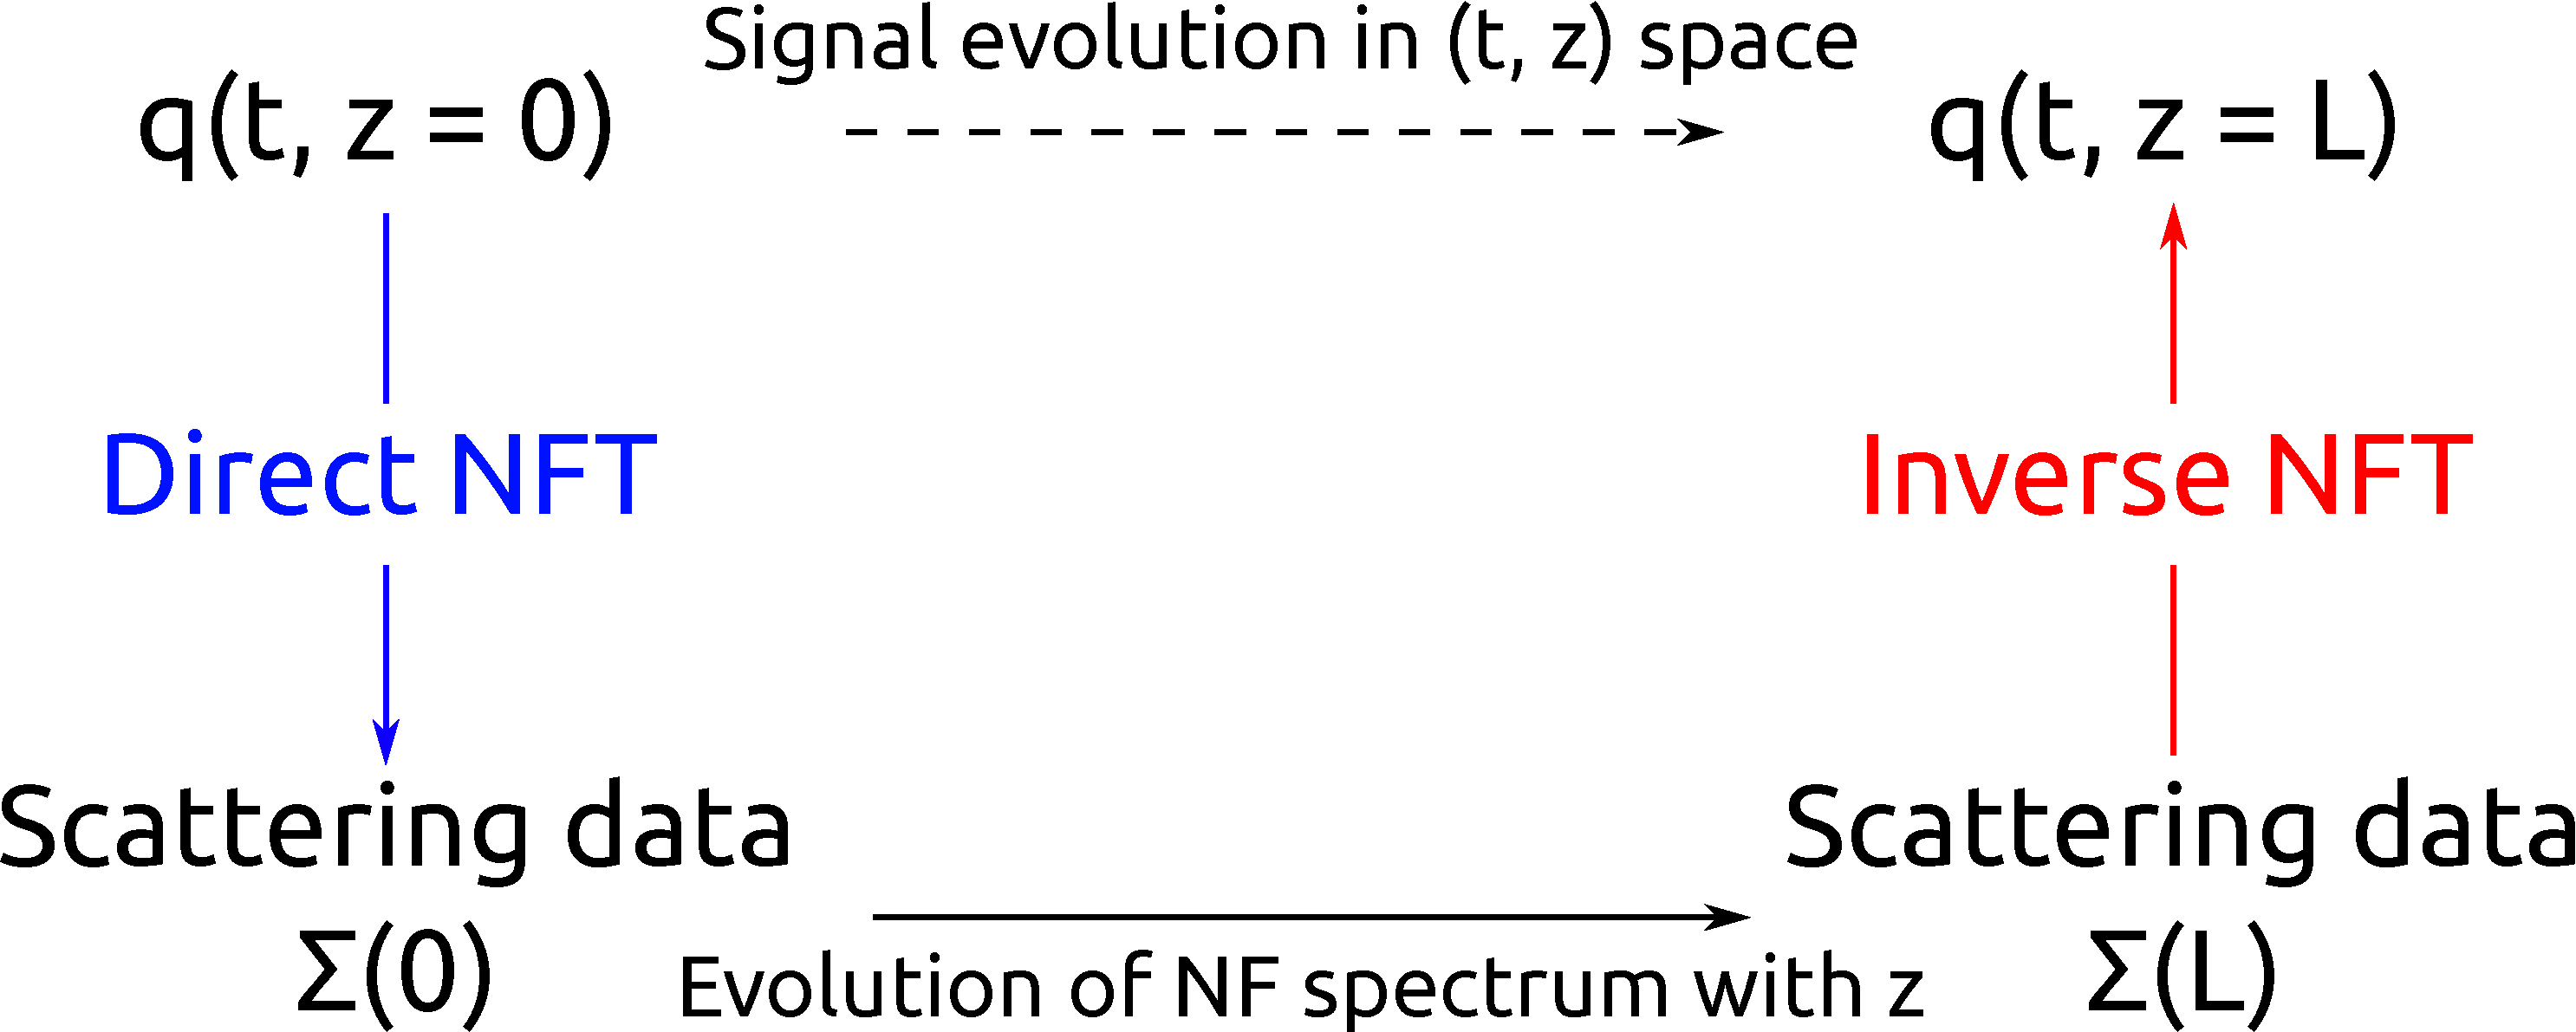
\includegraphics[width=0.7\linewidth]{images/theory/nft_scheme.pdf}
	\caption{Schematic representation of \acrlong{nft}.}
	\label{fig:IST}
\end{figure}


The \acrlong{nlse}~(\ref{eq:nlse_norm}) (so does \acrlong{me}~(\ref{eq:manakov_norm})) belongs to the class of the so-called integrable nonlinear partial differential equations that can be integrated by the \Gls{ist} method, also known as the nonlinear Fourier transform (NFT)~\cite{ZakharovShabat1972, Ablowitz1981}.
The \gls{nft} allows one to find the evolution (with $z$) of the signal $q(t,z)$ described by the \acrshort{nlse} channel by solving two linear problems instead of solving the nonlinear partial differential equation. A complex signal evolution governed by \acrshort{nlse} is replaced by 3 steps (see Fig.~\ref{fig:IST}):
\begin{enumerate}
    \item direct (linear) transform from $q(t,z=0)$ to the so-called scattering data $\Sigma(0)$ (nonlinear spectrum of the initial signal)
    \item trivial evolution of the nonlinear spectrum with z, and
    \item inverse (linear) transform to restore signal $q(t,z)$ at any desired propagation distance $z$.
\end{enumerate}
% We do describe here all mathematical details as they are comprehensively presented in \cite{Optica}. 
The \acrshort{nft} method is similar to standard Fourier approach for the solution of linear evolution equations: present initial field in the spectral domain, consider trivial evolution of each spectral harmonic, reconstruct evolved signal from the spectral components known for any propagation distance.


We will now focus on the \gls{nlse}~(\ref{eq:nlse_norm}) presented as:
\begin{equation}
    i \frac{\partial q}{\partial z} + \frac{\sigma}{2} \frac{\partial^2 q}{\partial t^2} + |q|^2 q = 0,
    \label{eq:nlse_norm_again}
\end{equation}
where \( q(t, z) \) represents the complex envelope of the optical field that decays rapidly as \( t \) approaches infinity. The variable \( z \) stands for the length of the optical fiber, and \( t \) is the time variable. The parameter \( \sigma \) takes a value of \( -1 \) for normal dispersion and \( 1 \) for anomalous dispersion~\cite{Agrawal2010}. This equation, set in a frame moving with the pulse, describes how light pulses \( q(t, z) \) travel through fiber optics. The initial conditions (Cauchy problem) for the pulse are set at a starting point \( z=z_0 \) and given by:
\begin{equation}
    q(t, z)|_{z=z_0} = q_0(t).
\end{equation}

The mathematical approach developed by Zakharov and Shabat~\cite{zakharov1972exact} integrates the \acrshort{nlse}. This technique, known as the \acrlong{nft}, converts the optical signal into a \acrfull{nf} spectrum. This spectrum is derived from the solutions to the \acrfull{zsp}.

Equation~(\ref{eq:nlse_norm_again}) can be written as a condition of compatibility:
\begin{equation}
    \frac{\partial L}{\partial z} = ML - LM,
\end{equation}
which are written as
\begin{equation}
    L\Psi = \xi \Psi, \quad \frac{\partial \Psi}{\partial z} = M\Psi,
    \label{eq:lax_pair_nlse}
\end{equation}
where \(\Psi(t)\) is a complex, two-component function that depends on the real variable \(t\), and
\begin{align}
    L = i \begin{pmatrix} \partial_t & -q \\ -\sigma q^* & -\partial_t \end{pmatrix}, \quad
    M = i \begin{pmatrix}  \sigma \partial_t^2 + \frac{1}{2} |q|^2  & -\sigma q \partial_t - \frac{1}{2} \sigma q_t \\
    -q^* \partial_t - \frac{1}{2} q_t & - \sigma \partial_t^2 - \frac{1}{2} |q|^2  \end{pmatrix}.
    \label{eq:nlse_l_and_m}
\end{align}
The first equation in Eq.~(\ref{eq:lax_pair_nlse}) is the eigenvalue problem for the operator \(L\). When \(\sigma = -1\), the operator \(L\) is Hermitian, meaning it equals its own complex conjugate transpose (\(L = L^\dagger = (L^*)^T\)), so the spectral parameter \(\xi = \zeta + i\eta\) is a real number \(\xi = \zeta\in \mathbb{R}\). If \(\sigma = 1\), there is no such constraint, and we find both continuous and discrete parts to the spectrum. The continuous part is on the real axe, while the discrete part is found where the imaginary part of \(\xi\) is greater than zero (\(\text{Im}(\xi) > 0\)).

The first equation in Eq.~(\ref{eq:lax_pair_nlse}) can also be expressed as an evolutionary system:
\begin{equation}
    \frac{d \Psi(t)}{dt} = Q(t)\Psi(t),
    \label{eq:zsp_matrix}
\end{equation}
where \(q = q(t, z)\) is the signal at any point \(z\) along the fiber, which we'll often not mention to simplify our equations. The vector \(\Psi(t)\) and the matrix \(Q(t)\) are defined as
\[
    \Psi(t) = \begin{pmatrix} \psi_1(t) \\ \psi_2(t) \end{pmatrix}, \quad Q(t) = \begin{pmatrix} -i \xi & q \\ -\sigma q^* & i \xi \end{pmatrix}.
\]
Some sources call this the \Gls{zssp}. When we look at the \gls{zssp} for the signal at the start of the fiber, \(q(t,z=0)\), the problem is laid out as:
\begin{equation}
\left\{
\begin{aligned}
	- \partial_{t} \psi_1 + q_0(t) \psi_2 = i \xi \psi_1, \\
	\partial_{t} \psi_2 + \sigma q_0^{*}(t) \psi_1 = i \xi \psi_2. \\
\end{aligned}
\right.
\label{eq:ZS}
\end{equation}
In these equations, \(q_0(t)\) is our initial signal, and \(\xi\) is a complex parameter that we use to solve the system.


% Also the first Eq. in Eq. (\ref{eq:lax_pair_nlse})  can be rewritten as an evolutionary system
% \begin{equation}
%     \frac{d \Psi(t)}{dt} = Q(t)\Psi(t),
%     \label{eq:zsp_matrix}
% \end{equation}
% where \(q = q(t, z)\) and
% \[
%     \Psi(t) = \begin{pmatrix} \psi_1(t) \\ \psi_2(t) \end{pmatrix}, \quad Q(t) = \begin{pmatrix} -i \xi & q \\ -\sigma q^* & i \xi \end{pmatrix}.
% \]
% Here \(z\) is a parameter, that we will skip further.

% In some literature the same problem referred as the \Gls{zssp}. We consider here \gls{zssp} problem for the initial signal $q(t,z=0)$: 
% \begin{equation}
% \left\{
% \begin{aligned}
% 	- \partial_{t} \psi_1 + q_0(t) \psi_2 = i \xi \psi_1 \\
% 	\partial_{t} \psi_2 + q_0^{*}(t) \psi_1 = i \xi \psi_2 \\
% \end{aligned}
% \right.
% \label{eq:ZS}
% \end{equation}

The system described by Eq.~(\ref{eq:zsp_matrix}) can also be expressed in a gradient form:
\begin{equation}
    \begin{pmatrix} \psi_1 \\ \psi_2 \end{pmatrix}_t
    = J \begin{pmatrix} \frac{\partial H}{\partial \psi_1^*} \\ \frac{\partial H}{\partial \psi_2^*} \end{pmatrix}
    = J \begin{pmatrix} -i \xi & \sigma q \\ -\sigma q^* & i \xi \end{pmatrix},
    \label{eq:nlse_jost_matrix}
\end{equation}
where \( H \) represents the energy of the system and is given by \( H = |\psi_1|^2 + \sigma |\psi_2|^2 \). When the spectral parameter \( \xi \) is a real number, the matrix \( J \) becomes skew-Hermitian (which means \( J = -J^* \)), and this applies for both values of \( \sigma = \pm 1 \). Therefore, the equation in (\ref{eq:nlse_jost_matrix}) keeps the value of \( H \) constant over time.

We can express the energy \( H \) and the matrix \( Q \) using special matrices called Pauli matrices, denoted as \( \sigma_0 \) and \( \sigma_3 \):
\begin{align}
    H &= \begin{cases} (\Psi^*, \sigma_0 \Psi), & \text{for } \sigma = 1, \\ (\Psi^*, \sigma_3 \Psi), & \text{for } \sigma = -1, \end{cases} \\
    Q &= \begin{cases} J \sigma_0, & \text{for } \sigma = 1, \\ J \sigma_3, & \text{for } \sigma = -1, \end{cases},
\end{align}
where the curved brackets \( (\cdot, \cdot) \) represent the scalar product of complex vectors.


% The system Eq.~(\ref{eq:zsp_matrix}) can be written in a gradient form as follows:
% \begin{equation}
%     \begin{pmatrix} \psi_1 \\ \psi_2 \end{pmatrix}_t
%     = J \begin{pmatrix} \frac{\partial H}{\partial \psi_1^*} \\ \frac{\partial H}{\partial \psi_2^*} \end{pmatrix}
%     = J \begin{pmatrix} -i \xi & \sigma q \\ -\sigma q^* & i \xi \end{pmatrix},
%     \label{eq:nlse_jost_matrix}
% \end{equation}
% where \( H = |\psi_1|^2 + \sigma |\psi_2|^2 \). For real spectral parameters \( \xi = \eta \) the matrix \( J \) is skew-Hermitian \( J = -J^* \) for any \( \sigma = \pm 1 \) and, consequently, the system Eq.~(\ref{eq:nlse_jost_matrix}) conserves the quadratic form \( H \).

% The invariant \( H \) and the matrix \( Q \) can be written using Pauli matrices \( \sigma_0 \) and \( \sigma_3 \) (see Appendix) as follows:
% \begin{align}
%     H &= \begin{cases} (\Psi^*, \sigma_0 \Psi), & \text{for } \sigma = 1 \\ (\Psi^*, \sigma_3 \Psi), & \text{for } \sigma = -1 \end{cases}, \\
%     Q &= \begin{cases} J \sigma_0, & \text{for } \sigma = 1 \\ J \sigma_3, & \text{for } \sigma = -1 \end{cases},
% \end{align}
% where the curved bracket indicate the scalar product of the complex vectors.

When the signal \( q(t) \) decays rapidly as \( t \) goes to infinity, we can find specific solutions, known as Jost functions, for the \acrshort{zsp} shown in Eq.~(\ref{eq:lax_pair_nlse}). These solutions are:
\begin{equation}
    \Psi = \begin{pmatrix} \psi_1 \\ \psi_2 \end{pmatrix}
    = \begin{pmatrix} e^{-i \xi t} \\ 0 \end{pmatrix} [1 + o(1)], \quad t \to -\infty,
    \label{eq:lax_left}
\end{equation}
for the left boundary, and
\begin{equation}
    \Phi = \begin{pmatrix} \phi_1 \\ \phi_2 \end{pmatrix} = \begin{pmatrix} 0 \\ e^{i \xi t} \end{pmatrix} [1 + o(1)], \quad t \to \infty,
    \label{eq:lax_right}
\end{equation}
for the right boundary. If we use the left boundary condition in Eq.~(\ref{eq:lax_left}), we can say that \( H = 1 \) for any real spectral parameter. From here, we can find the Jost scattering coefficients \(a(\xi)\) and \(b(\xi)\):
\begin{equation}
    a(\xi) = \lim_{t \to -\infty} \psi_1(t, \xi) e^{i \xi t}, \quad b(\xi) = \lim_{t \to -\infty} \psi_2(t, \xi) e^{-i \xi t}.
    \label{eq:nlse_ab}
\end{equation}
These coefficients always meet the following condition:
\begin{equation}
|a(\xi)|^2 + \sigma|b(\xi)|^2 \equiv 1.
\label{eq:quad_inv}
\end{equation}
The spectral data of the \acrshort{zsp} is given by \(a(\xi)\) and \(b(\xi)\) and can be described as:
\begin{enumerate}
    \item The zeros of \(a(\xi) = 0\) give us the discrete spectrum \(\{\xi_k\}, k = 0, K - 1\),
    with the phase coefficients defined by
    \begin{equation}
        r_k = \frac{b(\xi)}{a'(\xi)} \Bigg|_{\xi=\xi_k}, \quad \text{where } a'(\xi) = \frac{da(\xi)}{d \xi}.
        \label{eq:nlse_rk}
    \end{equation}
    \item The continuous spectrum is defined by reflection coefficient 
    \begin{equation}
        r(\xi) = b(\xi)/a(\xi), \xi \in \mathbb{R} {.}
        \label{eq:nlse_r}
    \end{equation}
\end{enumerate}
We use the "left" boundary condition Eq.~(\ref{eq:lax_left}) to find these spectral data. Both the left and right conditions Eqs.~(\ref{eq:lax_left}) and (\ref{eq:lax_right}) are useful for figuring out the coefficient \(b(\xi_k)\) for the discrete part of the spectrum:
\begin{equation}
    \Psi(t, \xi_k) = \Phi(t, \xi_k)b(\xi_k).
\end{equation}



% Assuming that \( q(t) \) decays rapidly when \( t \to +\infty \), the specific solutions (Jost functions) for ZSP Eq. (\ref{eq:lax_pair_nlse}) can be derived as:
% \begin{equation}
%     \Psi = \begin{pmatrix} \psi_1 \\ \psi_2 \end{pmatrix}
%     = \begin{pmatrix} e^{-i \xi t} \\ 0 \end{pmatrix} [1 + o(1)], \quad t \to -\infty,
%     \label{eq:lax_left}
% \end{equation}
% and
% \begin{equation}
%     \Phi = \begin{pmatrix} \phi_1 \\ \phi_2 \end{pmatrix} = \begin{pmatrix} 0 \\ e^{i \xi t} \end{pmatrix} [1 + o(1)], \quad t \to \infty,
%     \label{eq:lax_right}
% \end{equation}
% Taking into account the boundary conditions Eq.~(\ref{eq:lax_left}), we get the condition \( H = 1 \) for real spectral parameters. Then we obtain the Jost scattering coefficients \(a(\xi)\) and \(b(\xi)\) as follows:
% \begin{equation}
%     a(\xi) = \lim_{t \to -\infty} \psi_1(t, \xi) e^{i \xi t}, \quad b(\xi) = \lim_{t \to -\infty} \psi_2(t, \xi) e^{-i \xi t}.
% \end{equation}
% The scattering coefficients satisfy:
% \begin{equation}
% |a(\xi)|^2 + \sigma|b(\xi)|^2 \equiv 1.
% \label{eq:quad_inv}
% \end{equation}
% The spectral data of ZSP Eq. (\ref{eq:lax_pair_nlse}) are determined by \(a(\xi)\) and \(b(\xi)\) in the following way:
% \begin{enumerate}
%     \item \(K\) zeros of \(a(\xi) = 0\) define the discrete spectrum \(\{\xi_k\}, k = 0, K - 1\) of ZSP Eq. (5) and phase coefficients
%     \[
%         r_k = \frac{b(\xi)}{a'(\xi)} \Bigg|_{\xi=\xi_k}, \quad \text{where } a'(\xi) = \frac{da(\xi)}{d \xi}.
%     \]
%     \item the continuous spectrum is determined by the reflection coefficient \(r(\xi) = b(\xi)/a(\xi), \xi \in \mathbb{R}\).
% \end{enumerate}
% These spectral data were defined using the "left" boundary condition Eq. (\ref{eq:lax_left}). Both conditions Eqs. (\ref{eq:lax_left}) and (\ref{eq:lax_right}) can be used to calculate the coefficient \(b(\xi_k)\) of the discrete spectrum:
% \begin{equation}
%     \Psi(t, \xi_k) = \Phi(t, \xi_k)b(\xi_k).
% \end{equation}


The trace formula is given as~\cite{Ablowitz1981}:
\begin{equation}
    C_n = - \frac{1}{\pi} \int_{-\infty}^{\infty} (2i \xi)^n \ln |a(\xi)|^2 d \xi + \sum_{k=0}^{K-1} \frac{1}{n+1} \left[ (2i \xi_k^*)^{n+1} - (2i \xi_k)^{n+1} \right],
    \label{eq:nlse_cn}
\end{equation}
This formula links the NLSE integrals \(C_n\) with the scattering coefficient \(a(\xi)\) and the set of discrete spectral values \(\xi_k\). The integrals \(C_n\) are represented as:
\[
    C_0 = \int_{-\infty}^{\infty} |q|^2 dt, \, C_1 = \int_{-\infty}^{\infty} qq_t^* dt, \, C_2 = \int_{-\infty}^{\infty} (qq_{tt}^* + |q|^4) dt,
\]
\[
    C_3 = \int_{-\infty}^{\infty} (qq^*_{ttt} + 4|q|^2 qq^*_t + |q|^2 q^* q_t) dt.
\]
Specifically, Eq.~(\ref{eq:nlse_cn}) for \(n = 0\) yields:
\begin{equation}
    C_0 = - \frac{1}{\pi} \int_{-\infty}^{\infty} \ln |a(\xi)|^2 d \xi + \sum_{k=0}^{K-1} 2i (\xi_k^* - \xi_k),
    \label{eq:nlse_c0}
\end{equation}
This result is known as the Parseval equality for \acrshort{nlse} and it helps confirm the accuracy of numerical solutions by checking the balance between continuous and discrete spectral energies. The first term on the right in Eq.~(\ref{eq:nlse_c0}) is the energy from the continuous spectrum:
\begin{equation}
    E_c = - \frac{1}{\pi} \int_{-\infty}^{\infty} \ln |a(\xi)|^2 d \xi,
    \label{eq:nlse_e_cont}
\end{equation}
while the energy from the discrete spectrum is:
\begin{equation}
    E_d = \sum_{k=0}^{K-1} 2i (\xi_k^* - \xi_k).
    \label{eq:nlse_e_discr}
\end{equation}



% In addition, the following trace formula is valid~\cite{Ablowitz1981}:
% \begin{equation}
%     C_n = - \frac{1}{\pi} \int_{-\infty}^{\infty} (2i \xi)^n \ln |a(\xi)|^2 d \xi + \sum_{k=0}^{K-1} \frac{1}{n+1} \left[ (2i \xi_k^*)^{n+1} - (2i \xi_k)^{n+1} \right],
%     \label{eq:nlse_cn}
% \end{equation}
% which connects the NLSE integrals \(C_n\) with the coefficient \(a(\xi)\) and the discrete spectrum \(\xi_k\). The first integrals have the form
% \[
%     C_0 = \int_{-\infty}^{\infty} |q|^2 dt, \, C_1 = \int_{-\infty}^{\infty} qq_t^* dt, \, C_2 = \int_{-\infty}^{\infty} (qq_{tt}^* + |q|^4) dt,
% \]
% \[
%     C_3 = \int_{-\infty}^{\infty} (qq^*_{ttt} + 4|q|^2 qq^*_t + |q|^2 q^* q_t) dt.
% \]
% Equation~(\ref{eq:nlse_cn}) for \(n = 0\) gives
% \begin{equation}
%     C_0 = - \frac{1}{\pi} \int_{-\infty}^{\infty} \ln |a(\xi)|^2 d \xi + \sum_{k=0}^{K-1} 2i (\xi_k^* - \xi_k),
%     \label{eq:nlse_c0}
% \end{equation}
% is called the Parseval nonlinear equality and is used to verify the numerical calculations and the consistency of the continuous and discrete spectra found. The first term on the right-hand side of Eq.~(\ref{eq:nlse_c0})
% refers to the continuous spectrum energy:
% \begin{equation}
%     E_c = - \frac{1}{\pi} \int_{-\infty}^{\infty} \ln |a(\xi)|^2 d \xi {,}
% \end{equation}
% and discrete spectrum energy:
% \begin{equation}
%     E_d = \sum_{k=0}^{K-1} 2i (\xi_k^* - \xi_k),
% \end{equation}


The way scattering data changes with the distance \( z \) is described by:
\begin{equation}
    r(\xi,z) = r(\xi,z_0) e^{-2i \xi^2 (z - z_0)}, \quad 
    r_k(z) = r_k(z_0) e^{-2i \xi_n^2 (z - z_0)}.
\end{equation}

The scattering data combines into the core \( \Sigma (z) \), which is a sum of the discrete and continuous parts of the nonlinear spectrum:
\begin{equation}
    \Sigma_{dis}(z) = \sum_{k = 0}^{K - 1} r_k(z) e^{-i \zeta_n z},
    \label{eq:kernel_sol}
\end{equation}
for the discrete part, and
\begin{equation}
    \Sigma_{con}(z) = \frac{1}{2\pi} \int_{-\infty}^{+\infty} d\xi r(\xi, z) e^{-i \xi z},
    \label{eq:kernel_rad}
\end{equation}
for the continuous part. Here \( N \) represents the total number of discrete eigenvalues in the signal.

The last part of working with the \gls{nft} involves reconstructing the signal from the scattering data. To get the signal \( q(t, z) \) back at a certain distance \( z \), we use the core \( \Sigma (z) \) in two integral equations, known as the \acrfull{glm} equations:
\begin{equation}
    \Theta_1^{*}(t,s)+\int_{-s}^{t} \Sigma(s+\tau) \Theta_2(t,\tau) d\tau = 0,
    \label{eq:glm_1}
\end{equation}
\begin{equation}
    -\Theta_2^{*}(t,s)+\int_{-s}^{t} \Sigma(s+\tau) \Theta_1(t,\tau) d\tau + \Sigma(t+s) = 0,
    \label{eq:glm_2}
\end{equation}
where \( -t \le s < t \) and \( 0 \le t \le T \), with $ \Sigma (t) \equiv \Sigma (z = 0, t) $. We solve for two functions, \( \Theta_1 \) and \( \Theta_2 \), using these equations. Once we find these functions, we can recover the signal using the straightforward formula:
\begin{equation}
    q(z,t) = -2 \Theta_2^{*}(t,t).
    \label{eq:glm_q}
\end{equation}



% The dependence of the scattering data on $z$ can be represented in the form:
% \begin{equation}
%     r(\xi,z) = r(\xi,z_0) e^{-2i \xi^2 (z - z_0)} {,} \quad 
%     r_k(z) = r_k(z_0) e^{-2i \xi_n^2 (z - z_0)} {.}
% \end{equation}

% The scattering data forms the core $ \Sigma (z) = \Sigma_{dis} (z) + \Sigma_{con} (z) $, sum of the discrete and continuous nonlinear spectra, where
% \begin{equation}
%     \Sigma_{dis}(z) = \sum_{k = 0}^{K - 1} r_k(z) e^{-i \zeta_n z} {,}
%     \label{eq:kernel_sol}
% \end{equation}
% \begin{equation}
%     \Sigma_{con}(z) = \frac{1}{2\pi} \int_{-\infty}^{+\infty} d\xi r(\xi, z) e^{-i \xi z} {.}
%     \label{eq:kernel_rad}
% \end{equation}
% Here $N$ is a total number of discrete eigenvalues in signal.

% The final step of the \gls{nft} is to restore the signal from the scatter data. In order to restore the signal $q (t, z)$ at the required point $z$, the obtained core $\Sigma (z)$ must be substituted into a pair of integral equations that are called \acrfull{glm} equations:
% \begin{equation}
%     \Theta_1^{*}(t,s)+\int_{-s}^{t} \Sigma(s+\tau) \Theta_2(t,\tau) d\tau = 0 {,}
%     \label{eq:glm_1}
% \end{equation}
% \begin{equation}
%     -\Theta_2^{*}(t,s)+\int_{-s}^{t} \Sigma(s+\tau) \Theta_1(t,\tau) d\tau + \Sigma(t+s) = 0 {,}
%     \label{eq:glm_2}
% \end{equation}
% where the parameters are within $ -t \le s <t $ and $ 0 \le t \le T $, $ \Sigma (t) \equiv \Sigma (z = 0, t) $. A pair of functions $\Theta_1$ and $\Theta_2$ constitute a solution to the \acrshort{glm} equations. After finding the functions $\Theta_1$ and $ \Theta_2 $, the signal is restored by
% simple formula
% \begin{equation}
%     q(z,t)= -2 \Theta_2^{*}(t,t) {.}
%     \label{eq:glm_q}
% \end{equation}


\subsubsection{\acrshort{nft} for \acrlong{me}}

In the same way we can define \acrlong{nft} for \acrlong{me}~(\ref{eq:manakov_norm}):
\begin{gather} 
i \frac{\partial q_x}{\partial \zeta} + \frac{\sigma}{2}\frac{\partial^2 q_x}{\partial \tau^2} +  \left(|q_x|^2 + |q_y|^2\right) q_x = 0, \nonumber \\
i \frac{\partial q_y}{\partial \zeta} + \frac{\sigma}{2}\frac{\partial^2 q_y}{\partial \tau^2} + \left(|q_x|^2 + |q_y|^2\right) q_y = 0.
\label{eq:manakov_norm_again}
\end{gather}

The Lax operators of the Manakov equation are given by 
\begin{align}
    L_{\text{M}} &= i\begin{pmatrix} \partial_t & -q_1 & -q_2 \\
    -\sigma q_1^* & -\partial_t & 0 \\
    -\sigma q_2^* & 0 & \partial_t \end{pmatrix}, \\
    M_{\text{M}} &= i\begin{pmatrix}  \sigma \partial^2_t +  \frac{1}{2} (|q_1|^2 - |q_2|^2) & -\sigma q_1 \partial_t - \frac{1}{2} \sigma  q_{1_t} & -\sigma q_2 \partial_t - \frac{1}{2} \sigma q_{2_t} \\
    - q_1^* \partial_t - \frac{1}{2} q_{1_t}^* & - \sigma \partial^2_t -  \frac{1}{2} (|q_1|^2 - |q_2|^2) & 0 \\
    - q_2^* \partial_t - \frac{1}{2} q_{2_t}^* & 0 & - \sigma \partial^2_t -  \frac{1}{2} (|q_1|^2 - |q_2|^2) \end{pmatrix}.
\end{align}
Eigenvalues are found by solving the eigenproblem
\begin{equation}
    L\Psi = \xi \Psi {,}
\end{equation}

Zakharov-Shabat system can be written for the Manakov's equations in the following way (Manakov-Zakharov-Shabat (MZS) problem):
\begin{equation}
\left\{
\begin{aligned}
	- \partial_{t} \psi_1 + q_1(t) \psi_2 + q_2(t) \psi_3 = i \xi \psi_1, \\
	\partial_{t} \psi_2 + \sigma q_1^{*}(t) \psi_1 = i \xi \psi_2. \\
 \partial_{t} \psi_3 + \sigma q_2^{*}(t) \psi_1 = i \xi \psi_3. \\
\end{aligned}
\right.
\label{eq:zs_manakov}
\end{equation}

By the analoge for NLSE ZS problem, the basis vectors for the eigenspace (the space of all eigenfunctions of $\mathbf{L}$) for \acrshort{me} are given by
$$
\Phi(t) \rightarrow\left[\begin{array}{ll}
0 & 0 \\
1 & 0 \\
0 & 1
\end{array}\right] \exp (j \xi t) \quad \text{and} \quad \bar{\Phi}(t) \rightarrow\left[\begin{array}{l}
1 \\
0 \\
0
\end{array}\right] \exp (-j \xi t) \quad \text { for } t \rightarrow \infty .
$$
The same can be done for the boundary $t \rightarrow-\infty$ and this leads to the eigenfunctions
$$
\begin{gathered}
\Psi(t) \rightarrow\left[\begin{array}{l}
1 \\
0 \\
0
\end{array}\right] \exp (-j \xi t) \quad \text { for } t \rightarrow-\infty, \\
\bar{\Psi}(t) \rightarrow\left[\begin{array}{ll}
0 & 0 \\
1 & 0 \\
0 & 1
\end{array}\right] \exp (j \xi t) \quad \text { for } t \rightarrow-\infty .
\end{gathered}
$$
We can select either the set of eigenfunctions at the boundary \( t \rightarrow \infty \), which are \( \Phi \) and \( \bar{\Phi} \), or the set at the boundary \( t \rightarrow -\infty \), which are \( \Psi \) and \( \bar{\Psi} \), to serve as the independent basis for the eigenvalue problem. Then, we can represent the other set using this chosen basis. We choose the eigenfunctions $\Phi, \bar{\Phi}$ as the basis:
\begin{equation}
\begin{aligned}
\label{CommonSolution}
& \Psi=\bar{\Phi} a(\xi)+\Phi b(\xi), \\
& \bar{\Psi}=\Phi \bar{a}(\xi)+\bar{\Phi} \bar{b}(\xi),
\end{aligned}
\end{equation}
with dimensions $a \in \mathbb{C}, \bar{a} \in \mathbb{C}^{2 \times 2}, b \in \mathbb{C}^{2 \times 1}$ and $\bar{b} \in \mathbb{C}^{1 \times 2}$. Just one pair of these coefficients, either \(a\) and \(b\) or \(\bar{a}\) and \(\bar{b}\), is sufficient to fully describe the signal. These coefficients, \(a(\xi)\) and \(b(\xi)\), known as the Nonlinear Fourier coefficients, depend on the spectral parameter \(\xi\) and the initial position \(z_0\), but they are independent of the time variable \(t\). This allows us to select the basis vectors at any time point we choose for calculating the Nonlinear Fourier coefficients. Let's select the time as it goes to infinity, \(t \rightarrow \infty\). We already know the values for \(\Phi\) and \(\bar{\Phi}\) at this time from the boundary conditions:
$$
\begin{aligned}
\lim _{t \rightarrow \infty} \Psi & =\lim _{t \rightarrow \infty}\left(\bar{\Phi} a(\xi)+\Phi b(\xi)\right) \\
& =\left[\begin{array}{c}
a(\xi) \\
0 \\
0
\end{array}\right] \exp (-j \xi t)+\left[\begin{array}{ll}
0 & 0 \\
1 & 0 \\
0 & 1
\end{array}\right]\left[\begin{array}{l}
b_{1}(\xi) \\
b_{2}(\xi)
\end{array}\right] \exp (j \xi t)
 =\left[\begin{array}{c}
a(\xi) \exp (-j \xi t) \\
b_{1}(\xi) \exp (j \xi t) \\
b_{2}(\xi) \exp (j \xi t)
\end{array}\right]
\end{aligned}
$$
We can determine \(\Psi\) as time approaches infinity (\(t \rightarrow \infty\)) using the boundary condition set as time approaches negative infinity (\(t \rightarrow -\infty\)). Consequently, all eigenvectors mentioned in~\eqref{CommonSolution} are known at the same point in time, specifically when \(t\) approaches infinity. To calculate the Nonlinear Fourier Transform (NFT) coefficients, we multiply both sides of the equation by either \(\exp (j \xi t)\) or \(\exp (-j \xi t)\), depending on whether we are finding the \(a\) coefficients or \(b_{1,2}\) coefficients, respectively. Then, we pick out the appropriate component from the resulting expressions:
$$
\begin{aligned}
\lim _{t \rightarrow \infty} \Psi \exp (j \xi t) & =\left[\begin{array}{c}
a(\xi) \exp (-j \xi t) \\
b_1(\xi) \exp (j \xi t) \\
b_2(\xi) \exp (j \xi t)
\end{array}\right] \exp (j \xi t) =\left[\begin{array}{c}
a(\xi) \\
b_1(\xi)(\exp (j \xi t))^2 \\
b_2(\xi)(\exp (j \xi t))^2
\end{array}\right]
\end{aligned}
$$
and
$$
\begin{aligned}
\lim _{t \rightarrow \infty} \Psi \exp (-j \xi t) & =\left[\begin{array}{c}
a(\xi) \exp (-j \xi t) \\
b_1(\xi) \exp (j \xi t) \\
b_2(\xi) \exp (j \xi t)
\end{array}\right] \exp (-j \xi t) =\left[\begin{array}{c}
a(\xi)(\exp (-j \xi t))^2 \\
b_1(\xi) \\
b_2(\xi)
\end{array}\right]
\end{aligned}
$$


The NFT coefficients are thus given by
$$
a(\xi)=\lim _{t \rightarrow \infty} \psi_1 \exp (j \xi t), \quad b_i(\xi)=\lim _{t \rightarrow \infty} \psi_{i+1} \exp (-j \xi t)
$$
And we can define the same spectral data:
\begin{itemize}
    \item The zeros of \(a(\xi) = 0\) give us the discrete spectrum \(\{\xi_k\}, k = 0, K - 1\),
    with the phase coefficients defined by
    \begin{equation}
        r_{k,i} = \frac{b_i(\xi)}{a'(\xi)} \Bigg|_{\xi=\xi_k}, \quad \text{where } a'(\xi) = \frac{da(\xi)}{d \xi}.
        \label{eq:manakov_rk}
    \end{equation}
    \item The continuous spectrum is defined by reflection coefficient 
    \begin{equation}
        r_i(\xi) = b_i(\xi)/a(\xi), \xi \in \mathbb{R} {.}
        \label{eq:manakov_r}
    \end{equation}
\end{itemize}

Finding the NFT coefficients comes down to solving the MZS system~\eqref{eq:zs_manakov}. This is a scattering problem: in solving~\eqref{eq:zs_manakov}, we analyze how the eigenfunctions are scattered from $t \rightarrow-\infty$ to $t \rightarrow \infty$. The NFT coefficients are therefore sometimes called the scattering coefficients. They capture the scattering data of $\mathbf{q}\left(z_0, t\right)$ and can also be collected in the socalled scattering matrix $\mathbf{S}(z, \xi)$. We can express~\eqref{CommonSolution} in terms of the scattering matrix as
$$
\left[\begin{array}{ll}
\Psi & \bar{\Psi}
\end{array}\right]=\left[\begin{array}{ll}
\bar{\Phi} & \Phi
\end{array}\right] \underbrace{\left[\begin{array}{cc}
a & \bar{b} \\
b & \bar{a}
\end{array}\right]}_{\mathbf{S}(x, \xi)}
$$

%
The inverse problem consists of recovering the potentials $\mathbf{q} = \{q_1(t), q_2(t)\}\in \mathbb{C}^{1\times2}$, where the time $t \in \mathbb{R}$, $\xi=\zeta+i \eta \in \mathbb{C}^{+}$, by left spectral data:
%
\begin{equation}
    \left\{\mathbf{r}(\xi),\left[\xi_{k}, \mathbf{r}_{k}\right]_{k=0}^{K-1}\right\}.
\end{equation}
$$
% \Sigma_{l}=\left\{\mathbf{l}(\xi),\left[\zeta_{n}, \mathbf{l}_{n}\right]_{n=1}^{N}\right\}, \quad \Sigma_{r}=\left\{\mathbf{r}(\xi),\left[\zeta_{n}, \mathbf{r}_{n}\right]_{n=1}^{N}\right\}.
$$
%
Here $K$ is the number of the solitons in the signal. The inverse problem is reduced to solving the left system of integral equations

\begin{equation}
\begin{aligned}
&\mathbf{\Theta}_{1}^{*}(t, s)+\int_{-\infty}^{t} \mathbf{\Theta}_{2}\left(t, t^{\prime}\right) \mathbf{\Sigma}\left(t^{\prime}+s\right) d t^{\prime}=0, \quad t \geq s \\
&\mp \mathbf{\Theta}_{2}^{*}(t, s)+\mathbf{\Sigma}(t+s)+\int_{-\infty}^{t} \mathbf{\Theta}_{1}\left(t, t^{\prime}\right) \mathbf{\Sigma}\left(t^{\prime}+s\right) d t^{\prime}=0
\end{aligned}
\label{eq:glm_left}
\end{equation}

where 2-dimensional kernels are defined for all real $t$ by

\begin{equation}
\mathbf{\Sigma}(z)=\frac{1}{2 \pi} \int_{-\infty}^{\infty} \mathbf{r}(\xi) e^{-i \xi z} d \xi-i \sum_{k=0}^{K-1} \mathbf{r}_{k} e^{-i \xi_{k} z}{.}
\end{equation}


After solving the system~(\ref{eq:glm_left}), the potential $\mathbf{q}(t)$ is restored by the formulas

$$
\mathbf{q}(t)=-2 \mathbf{\Theta}_{2}^{*}(t, t)
$$

% \subsection{Old}

% The NF spectrum associated to a given pulse $q(t)$ (we drop the dependence of our quantities on $z$ for simplicity) having a finite $L_1$ norm, is calculated using the solutions of the so-called Zakharov-Shabat spectral problem\cite{zs72,tplwfkd17,nmp84,yk14-1}. The latter is represented by the set of coupled ordinary differential equations written for two auxiliary functions $v_{1,2}$. Our signal to decompose, $q(t)$, enters into this set as an effective potential. We write down the Zakharov-Shabat problem (the focusing NLSE case) as \cite{zs72}:
% \begin{equation}
% \frac{d}{dt}
% \left(\begin{matrix}v_1(t, \xi)\\ v_2(t, \xi)\end{matrix}\right)
% =\left(\begin{matrix}-i\xi&q(t)\\ -\bar{q}(t)&i\xi\end{matrix}\right)
% \left(\begin{matrix}v_1(t, \xi)\\ v_2(t, \xi)\end{matrix}\right).
% \label{f:ZSode}
% \end{equation}
% In Eq.~(\ref{f:ZSode}),  $\xi$ is the (generally complex-valued) spectral parameter which plays the role of conventional Fourier frequency for integrable nonlinear PDEs. The overbar in Eq. (\ref{f:ZSode}) and below denotes the complex conjugates of corresponding quantities. To determine the NF spectrum associated with our profile $q(t)$, we need to find the special solution  $\Phi(t,\xi)$ of Eq. (\ref{f:ZSode}), called Jost function, imposing the special asymptotic condition at the trailing end of the pulse:
% \begin{equation}
% \Phi(t,\xi)\equiv\left(\begin{matrix}\phi_1\\ \phi_2\end{matrix}\right)
% \xrightarrow[t\rightarrow-\infty]{} \left(\begin{matrix}e^{-i\xi t}\\ 0\end{matrix}\right).
% \label{f:asy}
% \end{equation}
% The NF pulse decomposition consists in finding the continuous and discrete components of the NF spectrum associated with the localised signal $q(t)$. The core part of NFT is the calculation of scattering coefficients, $a(\xi) \in \mathbb{C}$ and $b(\xi) \in \mathbb{C}$, defined through the Jost solution $\Phi(t,\xi)$ as follows
% \begin{equation}
% a(\xi)=\lim_{t\rightarrow+\infty}\phi_1(t,\xi) e^{i\xi t},
% \qquad b(\xi)=\lim_{t \rightarrow+\infty}\phi_2(t,\xi) e^{-i\xi t},
% \label{f:ab}
% \end{equation}
% where $\xi \in \mathbb{R}$. The scattering coefficients for the focusing NLSE satisfy:
% \begin{equation}\label{norm}
% |a(\xi)|^2 + |b(\xi)|^2 \equiv 1.
% \end{equation}
% The continuous part of NF spectrum is generally defined by the ratio of quantities $b$ and $a$ from (\ref{f:asy}):
% \begin{equation}
% \label{r}
% r(\xi)=b(\xi)/a(\xi), \qquad r(\xi) \in \mathbb{C},
% \end{equation}
% where $r(\xi)$ is often refereed to as the reflection coefficient. $r(\xi)$  plays the role of the ordinary Fourier spectrum for nonlinear integrable PDEs and converges to the FT of our signal in the low-power (linear) limit; see more direct expressions below. 

% The discrete part of NF spectrum (the solitonic degrees of freedom) consists of the set of complex-valued pairs: $\{ \xi_n, c_n\}$, where $n$ numerates the soliton mode, and each $\xi_n$ is the (non-degenerate) solution of the equation $a(\xi)=0$, laying the the upper complex semi-plane of $\xi$. The second quantity, the so-called norming constants $c_n$, are given (for a sufficiently localised signal\cite{vps19}) by: $c_n = c(\xi_n) = b(\xi_n)/a'(\xi_n)$, with prime meaning the derivative with respect to $\xi$. The value of $\xi_n$ determines the amplitude and frequency of each solitonic component, while $c_n$ defines the values of phase and the ``centre-of-mass''  position of a solitary mode. However, the discrete part of NF spectrum is not addressed in our study; see Refs.\cite{jgy18,ymm19,wxz20} where the solitonic parameters are computed using the NNs. 

% More exact mathematical details regarding the NF spectrum definition and properties can be found in, e.g., monograph \cite{nmp84}, see also Ref.~\cite{vps19} for a brief mathematical review.



% We briefly remind in this section basics of the inverse scattering method~\cite{ZakharovShabat1972}.
% % Channel description

% % Signal propagation is modelled by the nonlinear Schr\"odinger equation (in the scalar case, when the signal is transmitted through single polarization):

% % \begin{equation}
% % 	i \frac{\partial Q}{\partial Z} - \frac{\beta_2}{2} \frac{\partial^2 Q}{\partial T^2} + \gamma |Q|^2 Q = 0 {.}
% %     \label{eq:GNLSE}
% % \end{equation}
% % Here $Q$ is a complex envelope field that describes the optical signal, $Z$ is a distance (e.g. in $km$), $T$ is time (e.g. in $ps$), $\beta_2$ (in $ps^2/km$) is the group velocity dispersion parameter and $\gamma$ (in $W^{-1} km^{-1}$) is the nonlinear Kerr coefficient.


For most cases in this work we will use \acrshort{nft} for \acrshort{nlse}.


\subsection{Solitons}
The history of solitons begins in fact in 1834, when James Scott Russell observed a solitary shaft of water in a channel, moving without a noticeable change in shape or decrease in speed over several kilometers \cite{scott1844}. Such waves were called solitary, and later, in 1965, the term soliton was introduced to represent their particle-like essence \cite{zabusky1965}. However, even earlier, in 1831, M. Faraday \cite{faraday1831} described an effect in which a fine powder placed on an oscillating surface gathered in small "heaps"\ , which could be both stationary and moving. The properties of solitons were studied in the 1960s, when the inverse scattering method was introduced, in which solitons arose as separate solutions \cite{gardner1967}.

In the 20th century, autosolitons (dissipative solitons) were actively studied in physical, chemical, and biological systems. The main work on this topic is related to the reaction-diffusion model \cite{vasilyev1987en, kerner1991en}, which describes the localized structures that arise in the chemical reactions of activators, or in current flows in plasma, gas and semiconductors.

In nonlinear optics, solitons are divided into temporal and spatial. The temporal solitons are localized in time and related to optical pulses that retain their shape, and the spatial ones are self-directed beams, limited in transverse directions, orthogonal to the propagation vector. The formation and existence of such types of solitons is caused by the optical Kerr effect \cite{shen1984, butcher1990, boyd1992} --- a nonlinear change in the refractive index of the medium, depending on the light intensity and leading to spatial focusing (or defocusing) and temporal self-modulation phase.

Optical solitons are divided into two large classes: conservative and dissipative. Conservative solitons are created due to the balance of nonlinear focusing and linear spreading in transparent media in which there is no energy pumping, and the radiation loss is negligible. Dissipative solitons (autosolitons) are localized as a result of the balance of the inflow and outflow of energy in the system. For them, there may also be an effect of balancing linear spreading and nonlinear focusing.

% \begin{figure}
%     \begin{minipage}{0.48\linewidth}
%     \center{
%         \includegraphics[width=1.0\linewidth]{solit_f.png} a) \\
%     }
%     \end{minipage}
%     \hfill
%     \begin{minipage}{0.48\linewidth}
%     \center{
%         \includegraphics[width=1.0\linewidth]{solit_a.png} b) \\
%     }
%     \end{minipage}
%     \caption{Examples of soliton solution: a) --- fundamental soliton,
%     b) --- Akhmediev breather.}
%     \label{fig:solit}
% \end{figure}

These two classes of solitons have both common properties and fundamental differences, as a result of their common nature, but of a different method of formation. The set of basic parameters of dissipative solitons is discrete due to the requirement for the energy balance. This leads to their increased stability, and, as a result, dissipative solitons have prospects in various practical applications. Conservative solitons are determined by a continuously varying parameter, for example, intensity or width. Depending on the method of energy input into the optical system, the solitons are divided into coherent and incoherent. Coherent solitons are formed in a beam of continuous coherent radiation, which determines the frequency and phase. The incoherent signal forms incoherent solitons, for which the common radiation phase is arbitrary.

Due to the presence of noise in real systems, the possibility of spontaneous transition between soliton and soliton-free structures is realized. The soliton itself, although not a stable structure, can exist for a long time, since it is resistant to small perturbations. Transitions can be caused by large fluctuations that are unlikely in real systems. This fact leads to one interesting feature described in \cite{PS01}, when in the process of signal evolution in the system solitons arise.

The study of optical solitons began in the 60s of the 20th century, when the first optical nonlinear systems appeared, and experiments in this field became available. The first example was the article \cite{askaryan1962en} about the possibility of the existence of a spatial conservative soliton in a transparent medium with a self-focusing nonlinearity. Later, a time soliton was discovered in single-mode fibers with the Kerr nonlinearity \cite{hasegawa1973}.


\subsection{Analytical solutions}
\subsubsection{Satsuma-Yajima signal}

As the first analytical signal for which the nonlinear spectrum is known, we take the following:
\begin{equation}
    q(t, 0) = A \ \mathrm{sech}(t) {,}
    \label{eq:satsuma_yajima}
\end{equation}
hyperbolic profile with variable amplitude $ A $. We assume that $ A> 0 $ is real, because otherwise the phase factor only affects the phase of the solution $q (t, z)$, which in this context does not interest us. In 1974, Satsuma and Yajima showed that the signal~(\ref{eq:satsuma_yajima}) is a particular solution of the Zakharov-Shabat problem~(\ref{eq:ZS}), and its nonlinear spectrum was found.

They found that the function written as follows:
\begin{equation}
    \psi_1(t; \xi) =
    \begin{pmatrix}
        y_1^{(1)}(s; \xi) \\
        -A(\xi - \frac{1}{2}i)^{-1} y_1^{(2)}(s; -\xi) \\
    \end{pmatrix} {,}
\end{equation}
is the Jost function of the problem~(\ref{eq:ZS}), where the functions $ y_1^{(1,2)} $ are defined by:
\begin{equation}
    y_1^{(1)} (s; \xi) = s^{i\xi/2}(1 - s)^{-i\xi/2} F \left(-A, A, i\xi + \frac{1}{2}; s\right)
\end{equation}

\begin{equation}
    y_1^{(2)} (s; \xi) = s^{1/2 - i\xi/2}(1 - s)^{-i\xi/2} F \left(\frac{1}{2} - i\xi + A, \frac{1}{2} - i\xi - A, \frac{3}{2} - i\xi; s\right)
\end{equation}
in which $ F (\alpha, \beta, \gamma; s) $ is a hypergeometric function, $ s \equiv \frac{1 - \tanh (x)}{2} $.
Taking into account the properties of the hypergeometric function:
\begin{equation}
F(\alpha, \beta, \gamma; 0) = 1 \nonumber
\end{equation}
\begin{eqnarray}
F(\alpha, \beta, \gamma; s) = \frac{\Gamma(\gamma)\Gamma(\gamma - \alpha - \beta)}{\Gamma(\gamma - \alpha)\Gamma(\gamma - \beta)}F(\alpha, \beta, \alpha + \beta + 1 - \gamma; 1 - s) + \nonumber \\
+ \frac{\Gamma(\gamma)\Gamma(\alpha + \beta - \gamma)}{\Gamma(\alpha)\Gamma(\beta)}(1 - s)^{\gamma - \alpha - \beta}F(\gamma - \alpha, \gamma - \beta, 1 + \gamma - \alpha - \beta; 1 - s) \nonumber
\end{eqnarray}
it is easy to calculate the asymptotic behavior of the function $ \psi_1 (t; \xi) $:
\begin{equation}
    \psi_1(t; \xi) \to 
    \begin{pmatrix}
        1 \\
        0\\
    \end{pmatrix}
    e^{-i\xi t} {,} \qquad t \to \infty
\end{equation}
\begin{equation}
    \psi_1(t; \xi) \to 
    \begin{pmatrix}
        \frac{\Gamma^2(i\xi + \frac{1}{2})}{\Gamma(i\xi + \frac{1}{2} + A) \Gamma(i\xi + \frac{1}{2} -A)} e^{-i\xi t} \\
        -i \sin(\pi A) \mathrm{sech}(\pi \xi) e^{i\xi t} \\
    \end{pmatrix}
    {,} \qquad t \to -\infty
\end{equation}

The function
$\frac{\Gamma^2(i\xi + \frac{1}{2})}{\Gamma(i\xi + \frac{1}{2} + A) \Gamma(i\xi + \frac{1}{2} -A)}$
in front of $ e ^ {- i \xi t} $ in the last expression is nothing more than the coefficient $ a (\xi) $ whose zeros give us a discrete spectrum for problem~(\ref{eq:ZS}):
\begin{equation}
    \xi_n = i \left( A + \frac{1}{2} -n \right),
\end{equation}
where $ n $ is a positive integer satisfying the condition $ n <A + \frac{1}{2}$. The first eigenvalue appears at $ A = \frac{1}{2} $, the second at $ A = \frac{3}{2} $ and so on. Thus, for an arbitrary $ A> 0 $, the number of discrete eigenvalues is equal to the largest integer number $ n $ satisfying the condition $ n - \frac{1}{2} <A $.

\subsubsection{Rectangular pulse}

Another example of the initial distribution is a rectangular pulse with varying amplitude:
\begin{equation}
    q(t, 0) = \left\{
    \begin{aligned}
        A {,}& \quad 0 \leq t \leq 1 {,} \\
        0 {,}& \quad \text{otherwise} {.}
    \end{aligned} \right.
\end{equation}

Similarly, with the previous type of signal, we assume that $ A> 0 $ and real. The coefficient $ a (\xi) $ takes the form:
\begin{equation}
    a(\xi) = e^{i\xi} \left( \cos \sqrt{\xi^2 + A^2} - \frac{i\xi}{\sqrt{\xi^2 + A^2}}\sin \sqrt{\xi^2 + A^2} \right) {.}
\end{equation}
This expression is zero if the expression in parentheses is zero, which leads us to the transcendental equation:
\begin{equation}
    \cot \sqrt{\xi^2 + A^2} = \frac{i\xi}{\sqrt{\xi^2 + A^2}}
\end{equation}
This expression can be satisfied only for imaginary $ \xi $. Each subsequent eigenvalue appears when $ A = (n - \frac{1}{2}) \pi $, where $n$ is a positive integer. This formula can be rewritten as
\begin{equation}
    N = \mathrm{int}[1/2 + L_1(q)/\pi] {,}
    \label{eq:n_soliton_l1}
\end{equation}
where $ \mathrm{int} [...] $ means the integer part of the expression in brackets, and $N$ is the number of solitons.
The first level $L_1$ of the norm calculated by this formula is 1.57, the second is 4.71 and so on.

 

\subsection{NF spectrum associated with finite-extent signals}
In practical applications, we do not typically deal with the signals defined on the whole infinite $t$-axis, but rather operate with the truncated wave-forms, meaning that $q(t)$ is non-zero only inside the finite interval of $t$. In this case, the NF spectrum of the signal is completely characterised by the coefficient $b(\xi)$ from (\ref{eq:nlse_ab}), which becomes band-limited, appended with the finite discrete set of solitonic parameters $\{\xi_n,r_n\}$ \cite{gzl18,svp20}. When, in addition, the discrete NF spectrum is absent, as it is in the case considered, the whole NF spectrum can be defined using just $b(\xi)$ profile\cite{w17}, while the coefficient $a(\xi)$ can be expressed through $b(\xi)$ in the following way:
\begin{equation}\label{a-fin}
a(\xi) = \sqrt{1-|b(\xi)|^2} \, \exp \! \left[ \frac{i}{2 \pi} \intop^{\infty}_{-\infty} \frac{\ln \big(1-|b(s)|^2 \big)}{\xi - s} \, ds \right],
\end{equation}
where the integral in the exponent is understood in the principal value sense.
So, in practice, instead of $r(\xi)$ (\ref{eq:nlse_r}), it is sufficient to compute the b-coefficient, and then find $a(\xi)$ using Eq.~(\ref{a-fin}). If needed, we then can use both computed quantities to find the reflection coefficient (\ref{eq:nlse_r}). We note that within the b-modulation concept, which has turned out to be the most efficacious NFDM method developed so far, we utilise the $b(\xi)$ functions as information carriers\cite{w17,gzl18,svp20,cw20}.



\subsection{NF spectrum for the weakly-nonlinear case and threshold for soliton nucleation}
Let us assume that the amplitude of our signal is small, say $|q(t)| \sim \epsilon$, with $\epsilon \ll 1$. Then, we can derive the following expansions for the NF scattering coefficients \cite{pdt13}:
\begin{equation}\label{a1}
a(\xi) = 1 - \!\! \intop_{-\infty}^{\infty} \! dt_1 \!\! \intop_{-\infty}^{t_1} \!\! dt_2 \, e^{2 i \xi (t_1-t_2)} q(t_1) \bar q(t_2),
\end{equation}
up to $\epsilon^2$ (the next expansion term $\sim \epsilon^4$), and
\begin{equation}\label{b1}
b(\xi) = -\intop_{-\infty}^{\infty} \!\! dt_1 \, e^{- 2 i \xi t_1} \bar q(t_1) +  \!\! \intop_{-\infty}^{t} \!\! dt_1 \intop_{-\infty}^{t_1} \! \!dt_2 \!\! \intop_{0}^{t_2}\!\!  dt_3 \, e^{2 i \xi (t_2-t_1-t_3)} \bar q(t_1) q(t_2) \bar q(t_3),
\end{equation}
up to $\epsilon^3$  (the next expansion term $\sim \epsilon^5$). With the accuracy up to $\epsilon^4$, we have for the reflection coefficient:
\begin{equation}\label{r0}
r(\xi) = - \intop_{-\infty}^{\infty} \!\! dt_1 \, e^{- 2 i \xi t_1} \bar q(t_1) -  \intop_{-\infty}^{\infty} \!\! dt_1 \intop_{t_1}^{\infty} \! \!dt_2 \!\! \intop_{-\infty}^{t_2}\!\!  dt_3  \, e^{2 i \xi (t_2-t_1-t_3)} \bar q(t_1) q(t_2) \bar q(t_3) .
\end{equation}
So we see that the first linear term in $r(\xi)$ expansion is simply the conjugated FT of our signal up to the frequency scaling factor. Then, $r(\xi)$ from Eq.~(\ref{r0}) differs from the expression for $b(\xi)$, Eq.~(\ref{b1}), only by the terms $\sim \epsilon^3$ and higher, but the structure of both expressions is the same.